\documentclass[a4paper,12pt]{article} % тип документа

% report, book

% Рисунки
\usepackage{graphicx}
\usepackage{wrapfig}
\usepackage{mathtext}
\usepackage[left=2cm,right=2cm,
    top=2cm,bottom=2cm,bindingoffset=0cm]{geometry}

\usepackage{hyperref}
\usepackage[rgb]{xcolor}
\hypersetup{				% Гиперссылки
    colorlinks=true,       	% false: ссылки в рамках
	urlcolor=blue          % на URL
}

%  Русский язык

\usepackage[T2A]{fontenc}			% кодировка
\usepackage[utf8]{inputenc}			% кодировка исходного текста
\usepackage[english,russian]{babel}	% локализация и переносы


% Математика
\usepackage{amsmath,amsfonts,amssymb,amsthm,mathtools} 


\usepackage{wasysym}

\author{Анна Назарчук Б02-109}
\title{2.2.3 Измерение теплопроводности воздуха при атмосферном давлении}
\date{}
\begin{document}
\maketitle
\section{Аннотация}
В работе измеряется коэффициент теплопроводности воздуха, его зависимость от температуры по измерению нагрузочных прямых.
\textbf{Цель:} измерить коэффициент теплопроводности воздуха при атмосферном
давлении в зависимости от температуры.
\textbf{Оборудование:} цилиндрическая колба с натянутой по оси нитью; термостат;
вольтметр и амперметр (цифровые мультиметры); эталонное сопротивление; источник
постоянного напряжения; реостат (или магазин сопротивлений).
\section{Теоретические сведения}
Теплопроводность - это процесс передачи тепловой энергии от нагретых
частей системы к холодным за счёт хаотического движения частиц среды (молекул, атомов и т.п.). Закон Фурье:
\begin{equation}
\overrightarrow{q}=-\kappa\cdot \nabla T
\end{equation}
$\overrightarrow{q}$ - плотность потока энергии, $\kappa \backsim \lambda\bar{\upsilon}\cdot nc_v$ - коэффицент теплопроводности.
Для цилиндрической геометрии (рис. \ref{цилиндр})
\begin{figure}[h!]
\begin{center}
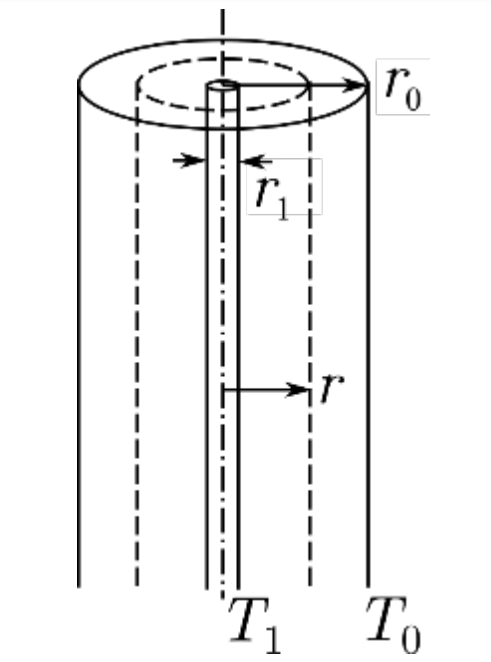
\includegraphics[width=0.3\textwidth]{Цилиндр}
\end{center}
\caption{Геометрия измерений} \label{цилиндр}
\end{figure}
Для стационарного режима и малого перепада температуры между нитью и стенками цилиндра:
\begin{equation}
Q = -2\pi r L\cdot \kappa \frac{dT}{dr}=\frac{2\pi L}{ln\frac{r_0}{r_1}}\kappa\cdot \Delta T
\end{equation}

\section{Экспериментальная установка и методика измерений}
Схема установки представлена на рис. \ref{схема}. Полость трубки заполнена воздухом при атмосферном давлении, металлическая нить - источник тепла и датчик температуры. Электрическая схема установки на рис. \ref{электричество}  
\begin{figure}[h!]
\begin{center}
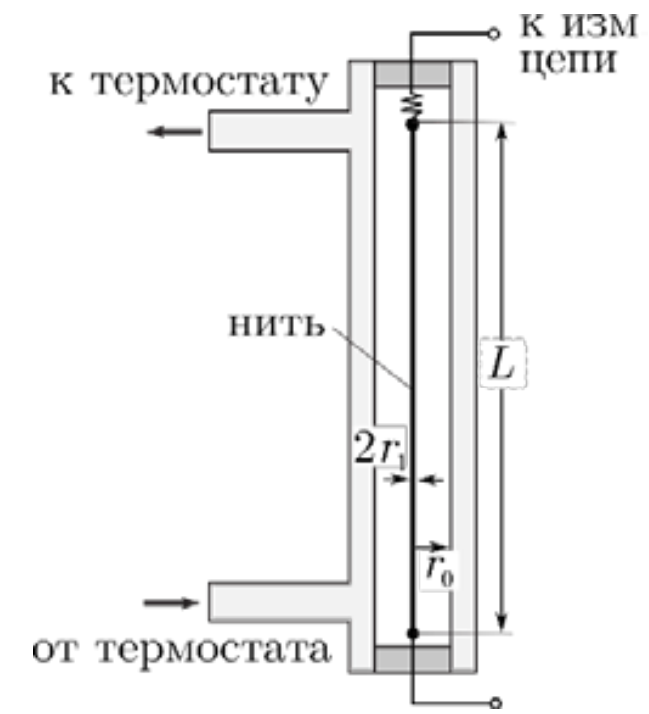
\includegraphics[width=0.3\textwidth]{Схема}
\end{center}
\caption{Схема установки} \label{схема}
\end{figure}

\begin{figure}[h!]
\begin{center}
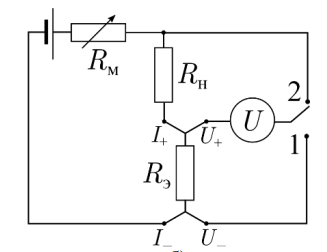
\includegraphics[width=0.3\textwidth]{Электричество}
\end{center}
\caption{Электрическая схема установки} \label{электричество}
\end{figure}
Ток цепи регулируется с помощью магазина сопротивлений, включенного последовательно с источником напряжения.

Измерение нагрузочных кривых позволяет получить температурную зависимость сопротивления нити (при $Q \to 0$, $T\approx T_0$)

Для исследуемых температур:
\begin{equation}
R(t)=R_{273}\cdot(1+\alpha t)
\end{equation}
$\alpha=\frac{1}{R_{273}}\frac{dR}{dT}$  - температурный коэффициент сопротивления материала. По наклонам нагрузочных кривых можно получить значение коэффициента теплопроводности.

\section{Измерения и обработка данных}
\begin{table}[h!]
\caption{Результаты измерений}
\label{результаты}
\begin{tabular}{|ll|ll|ll|}
\hline
\multicolumn{2}{|c|}{t=22$^\circ$C}     & \multicolumn{2}{c|}{t=30$^\circ$C}     & \multicolumn{2}{c|}{t=40$^\circ$C}     \\ \hline
\multicolumn{1}{|l|}{Uпр, мВ} & Uэт, мВ & \multicolumn{1}{l|}{Uпр, мВ} & Uэт, мВ & \multicolumn{1}{l|}{Uпр, мВ} & Uэт, мВ \\ \hline
\multicolumn{1}{|l|}{48.458}  & 83.609  & \multicolumn{1}{l|}{38.998}  & 69.951  & \multicolumn{1}{l|}{38.993}  & 69.462  \\ \hline
\multicolumn{1}{|l|}{55.121}  & 95.082  & \multicolumn{1}{l|}{48.415}  & 86.823  & \multicolumn{1}{l|}{55.069}  & 98.058  \\ \hline
\multicolumn{1}{|l|}{63.905}  & 110.31  & \multicolumn{1}{l|}{75.915}  & 136.11  & \multicolumn{1}{l|}{93.667}  & 166.69  \\ \hline
\multicolumn{1}{|l|}{122.43}  & 211.48  & \multicolumn{1}{l|}{122.16}  & 218.98  & \multicolumn{1}{l|}{175.82}  & 312.84  \\ \hline
\multicolumn{1}{|l|}{314.49}  & 543.87  & \multicolumn{1}{l|}{454.89}  & 813.74  & \multicolumn{1}{l|}{371.13}  & 660.41  \\ \hline
\multicolumn{1}{|l|}{409.95}  & 712.14  & \multicolumn{1}{l|}{588.65}  & 1051.2  & \multicolumn{1}{l|}{455.28}  & 810.79  \\ \hline
\multicolumn{1}{|l|}{514.64}  & 898.87  & \multicolumn{1}{l|}{689.69}  & 1232.7  & \multicolumn{1}{l|}{548.59}  & 979.77  \\ \hline
\multicolumn{1}{|l|}{551.61}  & 962.84  & \multicolumn{1}{l|}{833.58}  & 1458.1  & \multicolumn{1}{l|}{634.59}  & 1139.2  \\ \hline
\multicolumn{1}{|l|}{695.26}  & 1225.8  & \multicolumn{1}{l|}{}        &         & \multicolumn{1}{l|}{754.04}  & 1352.3  \\ \hline
\multicolumn{1}{|l|}{834.71}  & 1484.3  & \multicolumn{1}{l|}{}        &         & \multicolumn{1}{l|}{}        &         \\ \hline
\multicolumn{2}{|c|}{t=50$^\circ$C}     & \multicolumn{2}{c|}{t=60$^\circ$C}     & \multicolumn{2}{c|}{t=70$^\circ$C}     \\ \hline
\multicolumn{1}{|l|}{Uпр, мВ} & Uэт, мВ & \multicolumn{1}{l|}{Uпр, мВ} & Uэт, мВ & \multicolumn{1}{l|}{Uпр, мВ} & Uэт, мВ \\ \hline
\multicolumn{1}{|l|}{94.151}  & 163.66  & \multicolumn{1}{l|}{39.007}  & 68.255  & \multicolumn{1}{l|}{39.003}  & 69.451  \\ \hline
\multicolumn{1}{|l|}{314.15}  & 547.02  & \multicolumn{1}{l|}{55.096}  & 96.034  & \multicolumn{1}{l|}{55.081}  & 97.484  \\ \hline
\multicolumn{1}{|l|}{372.05}  & 648.51  & \multicolumn{1}{l|}{93.752}  & 163.11  & \multicolumn{1}{l|}{93.712}  & 165.53  \\ \hline
\multicolumn{1}{|l|}{457.08}  & 797.59  & \multicolumn{1}{l|}{176.08}  & 306.63  & \multicolumn{1}{l|}{175.92}  & 312.16  \\ \hline
\multicolumn{1}{|l|}{591.34}  & 1036.28 & \multicolumn{1}{l|}{313.95}  & 548.11  & \multicolumn{1}{l|}{313.21}  & 556.86  \\ \hline
\multicolumn{1}{|l|}{693.14}  & 1220.3  & \multicolumn{1}{l|}{410.21}  & 717.31  & \multicolumn{1}{l|}{408.75}  & 728.21  \\ \hline
\multicolumn{1}{|l|}{}        &         & \multicolumn{1}{l|}{515.41}  & 905.43  & \multicolumn{1}{l|}{513.55}  & 916.21  \\ \hline
\multicolumn{1}{|l|}{}        &         & \multicolumn{1}{l|}{590.71}  & 1041.4  & \multicolumn{1}{l|}{587.54}  & 1057.9  \\ \hline
\multicolumn{1}{|l|}{}        &         & \multicolumn{1}{l|}{691.78}  & 1226.2  & \multicolumn{1}{l|}{687.04}  & 1248.2  \\ \hline
\end{tabular}
\end{table}
Результаты измерений представлены в таблице \ref{результаты}.
Для не очень плохих температур построим график зависимости сопротивления нити от мощности. (рис. \ref{нагрузка}). Из графиков получаются следующие значения (табл. \ref{обработка})
\begin{figure}[h!]
\begin{center}
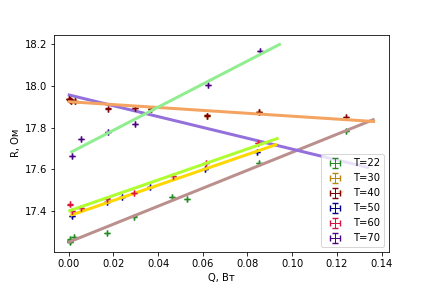
\includegraphics[width=\textwidth]{Нагрузка}\end{center}
\caption{Нагрузочные кривые для различных температур} \label{нагрузка}
\end{figure}

\begin{table}[h!]
\caption{Результаты обработки данных}
\label{обработка}
\begin{tabular}{|l|l|l|l|l|}
\hline
t, $^\circ$C & 22    & 50    & 60    & 70    \\ \hline
R/Q, Ом/Вт   & 17.25 & 17.38 & 17.40 & 17.68 \\ \hline
$\sigma_{R/Q}$, Ом/Вт  & 0.51  & 1.11  & 0.91  & 1.16  \\ \hline
$R_0$, Ом  & 4.32  & 3.69  & 3.74  & 5.55  \\ \hline
$\sigma_{R_0}$, Ом & 0.13  & 0.17  & 0.20  & 0.35  \\ \hline
\end{tabular}
\end{table}

Построим график зависимости сопротивления нити от её температуры (рис. \ref{R(T)})
\begin{figure}[h!]
\begin{center}
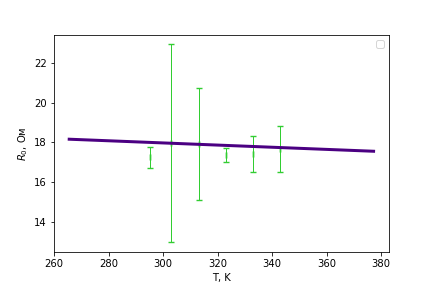
\includegraphics[width=\textwidth]{R(T)}\end{center}
\caption{Зависимость сопротивления от температуры} \label{R(T)}
\end{figure}
Погрешность на графике очень велика из-за плохих измерений напряжения на нити, то есть основной вклад в погрешность - линеаризация точек.

Из графика и линейной зависимости сопротивления от температуры найдем температурный коэффициент сопротивления:
\begin{equation}
\alpha=\frac{1}{R_{273}}\frac{dR}{dT}=(0.64 \pm 0.21)\cdot 10^{-3}  1/К
\end{equation}

Используя полученное значение и нагрузочные кривые, получим коэффицент теплопроводности для разных температур (табл. \ref{кси})

\begin{table}[h!]
\caption{Коэффициент теплопроводности для разных температур}
\label{кси}
\begin{tabular}{|l|l|l|l|l|}
\hline
t, $^\circ$C                     & 22   & 50    & 60   & 70   \\ \hline
$\kappa$, мВт/(м$\cdot$K)        & 7.34 & 8.59 & 8.51 & 5.71 \\ \hline
$\sigma_\kappa$, мВт/(м$\cdot$K) & 3.15 & 3.69  & 3.61 & 2.37 \\ \hline
\end{tabular}
\end{table}


Погрешности полученных значений огромны, что не позволяет сделать выводов о зависимости коэфициента теплопроводности от температуры.

\section{Выводы}

\hspace{5mm}
1. Получен линейных характер нагрузочных кривых, рассчитаны значения сопротивления при $Q=0$ и коэффицент наклона прямой.

2. Получен температурный коэффициент сопротивления: $\alpha=(0.74 \pm 0.21)\cdot 10^{-3}  1/К$.

3. Получены значения коэффицента теплопроводности воздуха при разных температурах, погрешности результатов не позволяют сделать выводы о температурных изменениях коэффициента теплопроводности.
\end{document}